\section{Sensor Nodes}

\begin{figure}[ht!]
   \centering
   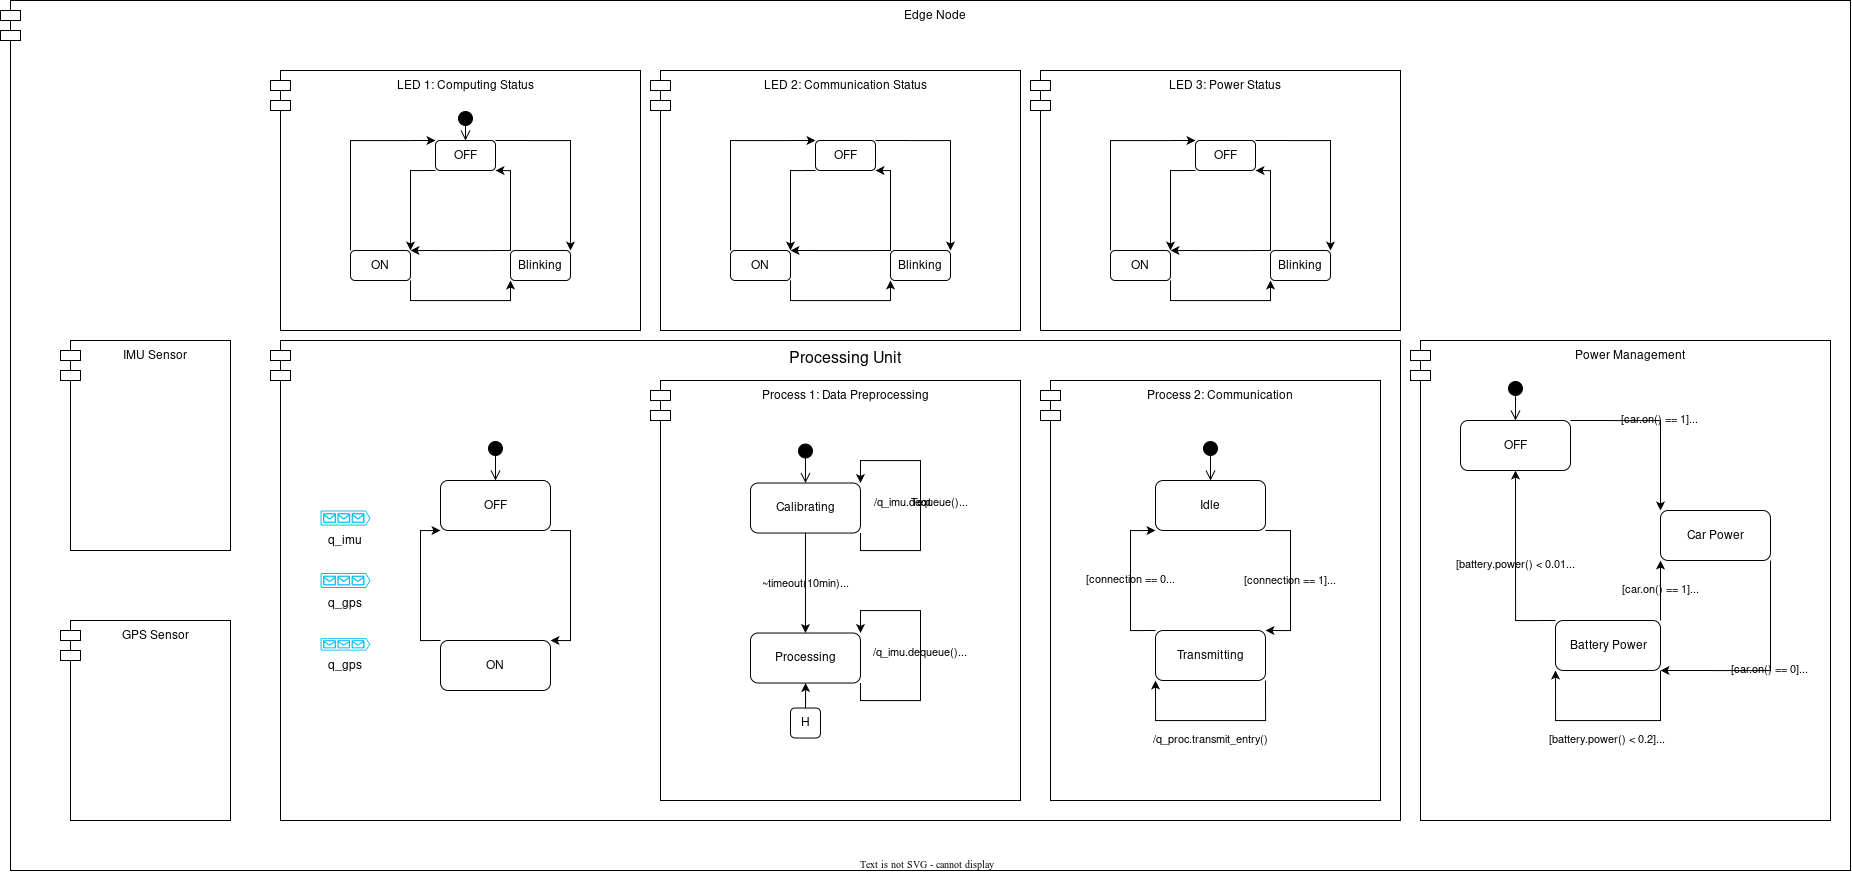
\includegraphics[width=\textwidth]{../../assets/diagrams/edge_node_rtuml/edge_node_rtuml.png}
   \hfill
   \caption{RT-UML of a Sensor Node}
   \label{fig:rt_uml_sensor_node}
\end{figure}

\begin{enumerate}
    \item \textbf{Cost Restriction per Node}: ~100 CHF \\
        Given the large number of vehicles that will host sensor nodes, the cost per node must remain as low as possible. To achieve this, each vehicle will have a single sensor node/package installed to minimize installation and part costs.

    \item \textbf{Quantification of Road State}: \\
        The sensor node will be ideally positioned centrally in the vehicle, above one of the axles, and securely mounted to the chassis to reduce measurement errors. The road state will be quantified on a scale from 0 (very good) to 244 (very poor), with 255 reserved for hazardous conditions.

    \item \textbf{Adaptation of Quantification to Vehicle Types and Driving Conditions}: \\
        A simple linear Mass-Spring-Damper model will be employed to account for the vehicle's influence on shock measurements while maintaining computational efficiency. An initial calibration phase, supported by default parameter settings, will adjust the model to fit the specific vehicle. During calibration, measured data will be mapped to quantified road state values. Additionally, other physical quantities beyond z-axis acceleration will be incorporated to decouple road state data from driving-induced accelerations.

    \item \textbf{High Polling Rate for IMU Measurements}: \\
        Road-induced shocks are brief and their period and amplitude are proportional to vehicle speed. The IMU's polling rate will be configured to ensure reliable readings for typical driving speeds.

    \item \textbf{Sensing of Physical Quantities}: \\
        The system will measure multiple physical quantities to ensure accurate road state assessments:
        \begin{enumerate}
            \item \textbf{Z-Axis Acceleration}: For detecting road conditions and potholes. Polling rate must adapt to vehicle velocity and be sufficiently high.
            \item \textbf{X- and Y-Axis Acceleration and Rotational Acceleration}: To minimize errors caused by driving dynamics.
            \item \textbf{Driving Velocity}: To correlate shock amplitudes with velocity using the Mass-Spring-Damper model.
            \item \textbf{Geographical Position}: To map road state measurements to specific locations.
        \end{enumerate}

    \item \textbf{Data Transmission at Established Gatepoints}: \\
        \begin{enumerate}
            \item \textbf{Data Format}: Each data package will include the following information encoded as a JSON object:
              \begin{lstlisting}[breaklines=true, basicstyle=\ttfamily]
(Node ID (2 Bytes)) | Position (2 x 8 Bytes (Double-Precision Float)) | Road Quality (1 Byte) | Unix Timestamp (4 Bytes)
              \end{lstlisting}

              For example, the following snippet represents a valid data sample in JSON format:

              \begin{lstlisting}[breaklines=true, basicstyle=\ttfamily]
{               
  "lat": 46.19313,
  "lon": 6.80421,
  "timestamp": 1734478933,
  "bumpiness": 50,
  "device_id": "USI-Car-1""
}
              \end{lstlisting}

            \item \textbf{Local Preprocessing}: The node will preprocess and store position-quality tuples locally.
            \item \textbf{Gatepoint Connectivity}: The node will automatically establish a connection at predefined gatepoints to transmit new data.
            \item \textbf{Data Protocol}: Data packages will be transmitted in MQTT format to a RabbitMQ server.
        \end{enumerate}
\end{enumerate}
